\chapter{Implementation Phase} \label{chap:implementation}

{This chapter introduces AMS integration and infrastructure followed by software architecture. It elaborates individual AMS commands and focuses also on documentation, both technical and for users. Big part of this chapter is dedicated to quality assurance, regarding recommended automatic testing, expert evaluation and user tests that have been done.}

\section{Integration and Infrastructure}\label{sec:intandinf}

{AMS is designed to be fully integrable with git-based repositories. It currently implements GitLab API and is GitHub forward-compatible (see Implementation Details). Similarly it can use various run environments, currently implementing GitLab CI.}

{Integrating AMS into an assignment uses a simple \texttt{include} statement with a URL. Thanks to git-flow branching model and semantic versioning (see Implementation Qualities) it is possible to determine a specific branch (stage or version).}

{GitLab CI introduces multiple variables that are overall optional. Among others, using variables you can specify a list of users (there are other ways to do so), automatic evaluation or set an evaluation due-date. For the full list of variables, see AMS specification (README).}

\begin{itemize}
\item
  {Git-based repository management systems, e.g. GitLab, GitHub.}
\item
  {Run environments, e.g. GitLab CI, GitHub Actions, Travis CI.}
\item
  {Simple integration into CI using variables}
\item
  {One click or automatic execution.}
\end{itemize}

\begin{figure}[H]
    \centering
    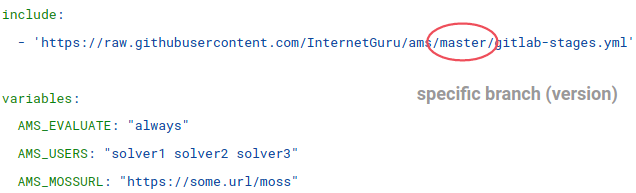
\includegraphics[width=\textwidth,height=\textheight,keepaspectratio]{Figures/impl/image7.png}
    \caption[Sample AMS integration into a GitLab project]{Sample AMS integration into a GitLab project containing an assignment. The given example illustrates AMS integration on a production stage (master branch), ergo the most current stable version available.}
\end{figure}

\subsection{Implementation Qualities}\label{ssec:implqaul}

\begin{itemize}
\item
  {Automatic tests using Bash unit testing tool}
\item
  {Follows Google shell style guide}
\item
  {Uses ShellCheck (a shell script static analysis tool)}
\item
  {Uses Semantic Versioning}
\item
  {Implements git-flow branching model}
\item
  {Ready to keep a changelog}
\end{itemize}

\subsection{Implementation Details}\label{sec:impldet}

\begin{itemize}
\item
  {Git commands extension \& normalization}
\item
  {Separate GitLab API (extendable)}
\item
  {Standard error code handling \& native Bash expansions}
\item
  {Options and arguments processed using getopt}
\item
  {Local variables \& constants, encapsulation}
\item
  {Conventional usage formatting}
\item
  {ns vs prefix}
\item
  {due date logic: do not close, commit vs push}
\item
  {git library}
\item
  {global environment for bash script}
\item
  {bash unit testing}
\item
  {due date concept (not closing)}
\end{itemize}

\section{Software Architecture}\label{sec:softarch}

{AMS is completely operable using CLI. Therefore it is integrable into any thinkable UI, such as a web browser. Imagine using GitLab's online editor (basic or advanced) on any device including smartphones \cite{10.1145/2325296.2325336}.}

{AMS can be operated locally using a terminal. As it is based on git, individual assignments can be developed and solved using any thinkable editor and environments, such as browser editors, terminal or IDE (such as Eclipse).}

{AMS script contains multiple sub-commands similarly to git, e.g. \texttt{git commit} or \texttt{git clone}. Each command has its own standard documentation including simple installation into \texttt{man pages}.}

\begin{itemize}
\item
  {CLI command based on Bash, Git and others.}
\item
  {Conventional README \& per-command documentation.}
\item
  {Documentation compiling into man pages using go-md2man.}
\item
  {AMS commands: distribute, evaluate, collect, measure.}
\item
  {AMS GitHub repository\footnote{https://github.com/InternetGuru/ams}}
\item
  {AMS Documentation\footnote{https://github.com/InternetGuru/ca/tree/dev/documentation}}
\item
  {AMS README\footnote{https://github.com/InternetGuru/ca/blob/dev/README.md}}
\end{itemize}

\begin{figure}[H]
    \centering
    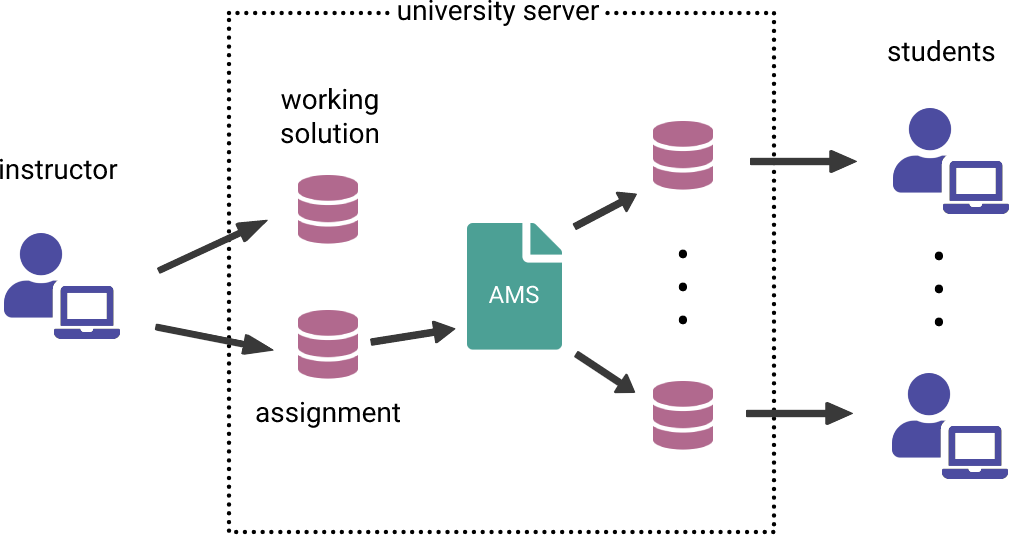
\includegraphics[width=0.8\textwidth,height=\textheight,keepaspectratio]{Figures/impl/image5.png}
    \caption[Distribution architecture diagram]{Distribution architecture shows an assignment being distributed from an instructor's repository among individual solvers. Similarly, if solvers' repositories already exist, the distribute command updates them.}
\end{figure}

\begin{figure}[H]
    \centering
    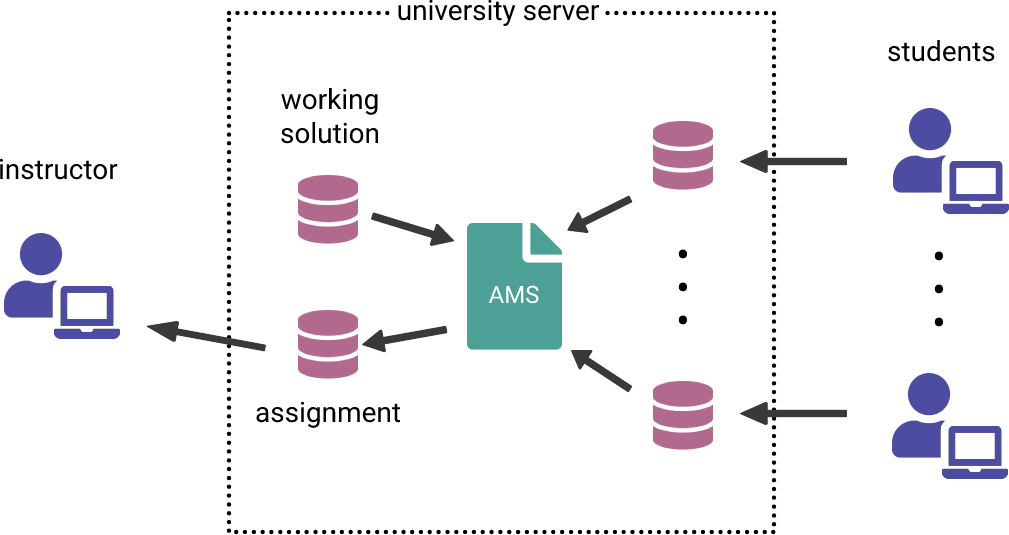
\includegraphics[width=0.8\textwidth,height=\textheight,keepaspectratio]{Figures/impl/image4.png}
    \caption[Collecting architecture diagram]{Collecting architecture is similar to the distribution architecture in the opposite direction. All solvers' repositories are collected and evaluated against the original working solution's tests and results provided to the instructor. Similarly does it work for measuring, where individual solutions are measured against each other.}
\end{figure}

\begin{figure}[H]
    \centering
    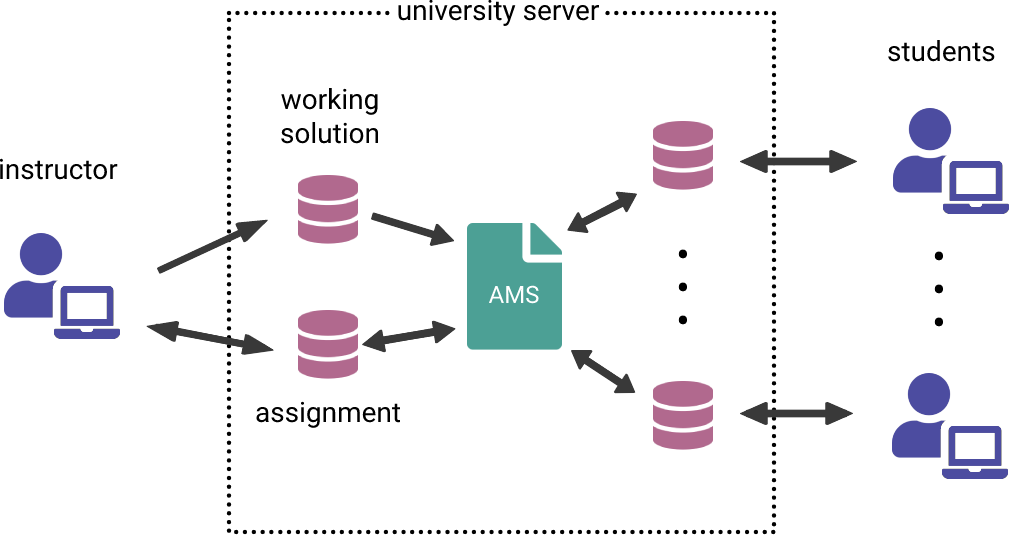
\includegraphics[width=0.8\textwidth,height=\textheight,keepaspectratio]{Figures/impl/image8.png}
    \caption[General software architecture diagram]{General software architecture shows both previous architectures combined. The message here is that any kind of execution (solving, distribution, updating, evaluation, measure) could be done at any point in time regardless.}
\end{figure}

\subsection{Distribute Command}\label{ssec:distribcmd}

\begin{itemize}
\item
  {Distributes an assignment among users.}
\item
  {Accepts user names from stdin.}
\item
  {Destination namespace and repository prefix.}
\item
  {Assigns existing users to the distributed assignments.}
\item
  {Distributes repository issues with a specific label.}
\item
  {Optionally updates repository links in README files.}
\item
  {AMS distribute command documentation\footnote{https://github.com/InternetGuru/ams/blob/dev/documentation/ams-distribute.md}}
\end{itemize}

\subsection{Evaluate Command}\label{ssec:evalcmd}

\begin{itemize}
\item
  {Evaluates code on compilation, coding style and automatic tests.}
\item
  {Uses Google Java Checkstyle, Apache Maven, Shields.io.}
\item
  {Creates log files with complete results to be displayed and linked.}
\item
  {Generates summary into files and colored status badges. (follows)}
\item
  {AMS evaluate command documentation\footnote{https://github.com/InternetGuru/ams/blob/dev/documentation/ams-evaluate.md}}
\end{itemize}

\begin{figure}[H]
    \centering
    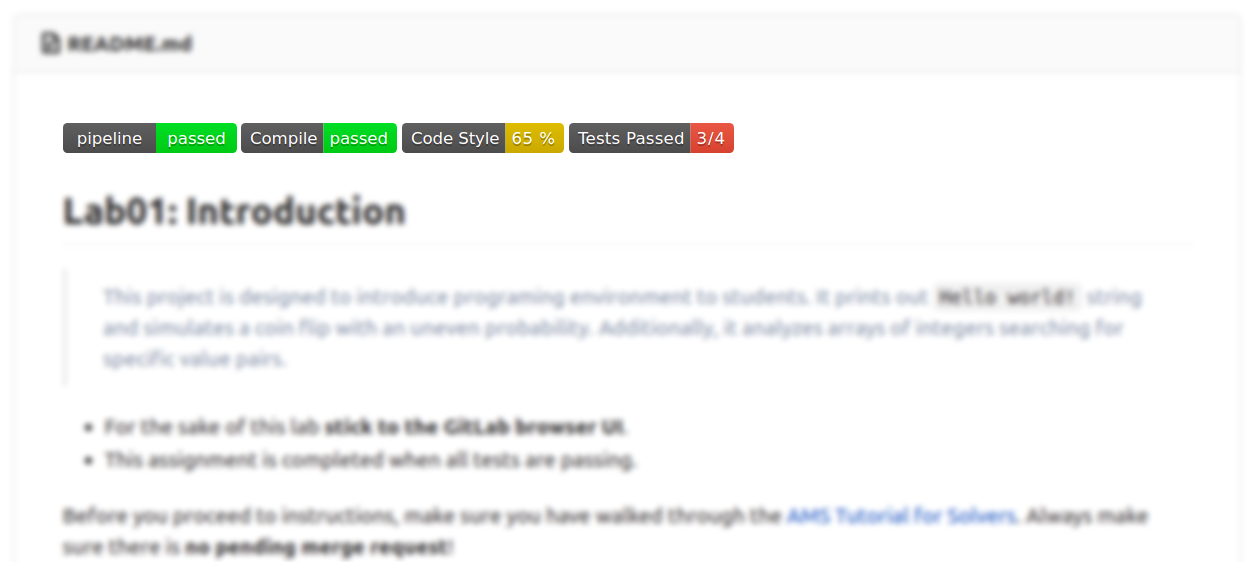
\includegraphics[width=\textwidth,height=\textheight,keepaspectratio]{Figures/impl/image1.png}
    \caption[Example status badges]{Status badges as they appear in each assignment, for individual solvers including the instructor's working assignment. Given example shows the code passing on compilation, matching only 65 \% of coding style and passing 3 tests out of 4.}
\end{figure}

\subsection{Collect Command}\label{ssec:collectcmd}

\begin{itemize}
\item
  {Clones assignments from a given namespace, e.g. semester.}
\item
  {Evaluates each assignment with AMS evaluate. (above)}
\item
  {Uses base files and (extended) tests from working project.}
\item
  {Supports evaluation to a specific date, e.g. deadline.}
\item
  {Creates summary with evaluation results. (follows)}
\item
  {AMS collect command documentation\footnote{https://github.com/InternetGuru/ams/blob/dev/documentation/ams-collect.md}}
\end{itemize}

\begin{figure}[H]
    \centering
    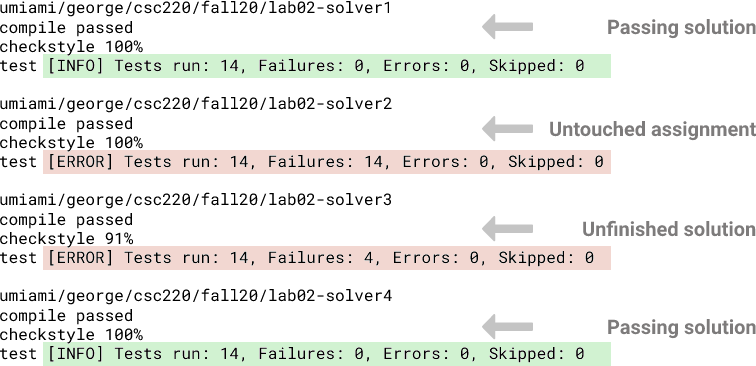
\includegraphics[width=\textwidth,height=\textheight,keepaspectratio]{Figures/impl/image2.png}
    \caption[Collective evaluation output example]{Sample illustration of collective evaluation output -\/- providing similar information to status badges (above). Given results show 4 users, where solver1 and solver4 have fully passing solutions, solver2 barely touched the assignment as 14 of 14 tests are failing. Finally, solver3 is passing 10 out of 14 tests.}
\end{figure}

\subsection{Measure Command}\label{ssec:measurecmd}

\begin{itemize}
\item
  {Measures software similarities using Moss (follows), potentially other metrics, e.g. SonarQube.}
\item
  {Uses original assignment as a base code.}
\item
  {Outputs link to Moss result page for further processing, e.g. manual browsing or visualization.}
\item
  {CI adds a working solution into the comparison.}
\item
  {AMS measure command documentation\footnote{https://github.com/InternetGuru/ams/blob/dev/documentation/ams-measure.md}}
\end{itemize}

\begin{figure}[H]
    \centering
    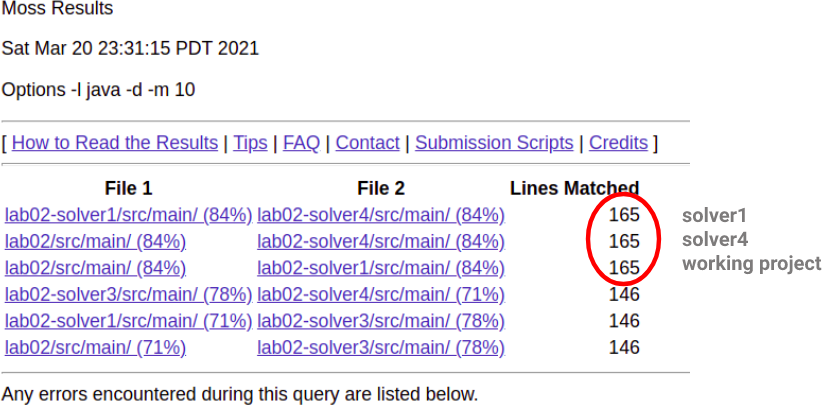
\includegraphics[width=\textwidth,height=\textheight,keepaspectratio]{Figures/impl/image3.png}
    \caption[Moss result page example]{Sample Moss result page ready to be explored or further analyzed / visualized by tools (below). Given example shows solver1 and solver4 having suspiciously similar solutions to each other and to the instructor's working solution.}
\end{figure}

\begin{figure}[H]
    \centering
    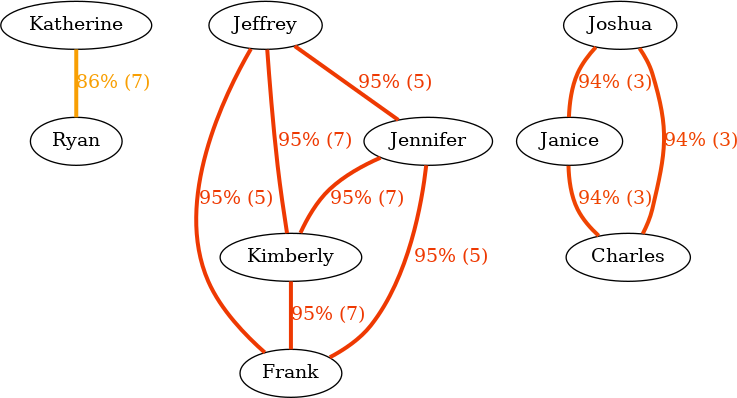
\includegraphics[width=\textwidth,height=\textheight,keepaspectratio]{Figures/impl/image6.png}
    \caption[Moss visualization example]{Sample Moss visualization (unrelated to sample result page provided above). It shows groups of students that might have been working on projects together weather it was planned for or not.}
\end{figure}

\subsection{Moss Plagiarism Types}\label{ssec:mossplagtyp}

{Stanford's Moss script has been implemented as one of the most sophisticated and favorized (and free) tools for software similarity measure purposes\cite{mosspaper}. It uses several types of plagiarism detection as indicated below. Above that it introduces noise suppression, base file and common passages.}

\begin{itemize}
\item
  {Type 1 refers to changing whitespace, layout, and comments.}
\item
  {Type 2 refers to changing types, identifiers, and literals.}
\item
  {Type 3 refers to reordering, adding, or removing statements.}
\item
  {Type 4 refers to refactoring the code to use different syntactic variants.}
\item
  {\#noise-suppression \#base-file \#common-passage}
\item
  {An article on How Moss Works\footnote{https://yangdanny97.github.io/blog/2019/05/03/MOSS}}
\end{itemize}

{It's worth noting, that based on the AMS integration, any other software can be easily integrated including existing commercial services or an own script.}

\section{Documentation}\label{sec:doc}

{There is a simple configuration and setup guide including basic instructions for maintenance. Technically, AMS is fully documented and additionally a couple of tutorials and sample labs is introduced -\/- on how to use the system as an instructor or solver (student).}

\subsection{Installation and Maintenance}\label{ssec:installandmaint}

{The current implementation requires GitLab instance with GitLab CI run environment, either publicly or on its own server. AMS will run on any bash-compatible environment with a set of basic commands (see documentation). In order to contribute, follow implementation qualities (above) or simply use the issue tracker in the project's repository.}

\begin{itemize}
\item
  {Requirements}
  \begin{itemize}
  \item
    {GitLab}
  \item
    {GitLab CI runner (own / with prepaid minutes)}
  \end{itemize}

\item
  {Installation}
  \begin{itemize}
  \item
    {Solver can easily integrate specific CI into the project, see Tutorial for Instructors below.}
  \item
    {Advanced users can install AMS script locally and use it from CLI by following man pages.}
  \end{itemize}

\item
  {How to contribute}
  \begin{itemize}
  \item
    {Fork AMS project on GitHub}
  \item
    {Proceed changes in forked project}
    \begin{itemize}
    \item
      {add new features / bug fixes on \texttt{dev} branch or}
    \item
      {add hotfix on \texttt{master} branch}
    \end{itemize}
  \item
    {In case of hotfixing increment patch version in \texttt{VERSION} file}
  \item
    {Summarize changes into \texttt{CHANGELOG.md} file following keep a changelog syntax}
  \item
    {Create new pull request to original project}
  \end{itemize}
\end{itemize}

\subsection{Technical Documentation}\label{ssec:techdoc}

{Above general \texttt{README}, all individual sub-commands as much as the AMS script has their own technical documentation. Individual files can be found in a \texttt{documenta\-tion} folder in its repository. Documentation files also serve as sources for generating usage and man pages.}

\begin{itemize}
\item
  {See project documentation folder\footnote{https://github.com/InternetGuru/ca/tree/dev/documentation} or APPENDIX \ref{apx:ams-documentation}.}
\item
  {Manual pages for every ca command (when installed locally)}
  \begin{itemize}
  \item
    {\texttt{man ams}}
  \item
    {\texttt{man ams-distribute}}
  \item
    {\texttt{man ams-collect}}
  \item
    {\texttt{man ams-evaluate}}
  \item
    {\texttt{man ams-measure}}
  \end{itemize}
\end{itemize}

\subsection{User Documentation and Sample Labs}\label{ssec:userdocandlabs}

{There is a separate tutorial for instructors on creating, distributing, collecting and measuring assignments. Similarly there is a tutorial for solvers on how to solve assignments. To illustrate and test both tutorials, there are two basic assignments inspired by the first two labs of Java programming course (CSC220).}

\begin{itemize}
\item
  {Tutorial for Instructors, see APPENDIX \ref{apx:tut-ins}}
\item
  {Tutorial for Solvers, see APPENDIX \ref{apx:tut-sol}}
\item
  {Lab1: Introduction, see APPENDIX \ref{apx:lab01}}
\item
  {Lab2: Matrix, see APPENDIX \ref{apx:lab02}}
\item
  {AMS README file, see APPENDIX \ref{apx:ams-readme}}
\end{itemize}

\section{Quality Assurance}\label{sec:qa}

{There is a series of recommended automatic tests and the environment (CI) is set to execute tests at each commit. As AMS is designed to have multiple non-expert users (including students), special attention has been granted to expert evaluation and user testing.}

\subsection{Automatic Testing}\label{ssec:autotest}

{To support current and future development, an automated testing environment is introduced. Following are sets of features to be checked for each and every change (commit). Starting with a general description -\/- how to check on options, variables and run code analysis.}

\begin{itemize}
\item
  {Script options (long and short) with valid and invalid values, e.g. invalid date, invalid file pattern}
\item
  {CI variables: default, invalid}
\item
  {Code analysis using Shellcheck.}
\end{itemize}

\subsubsection{Test ams script}

\begin{itemize}
\item
  {Valid and invalid working dir}
\item
  {Valid and invalid command}
\item
  {Missing requirements (jq, git)}
\item
  {Access token - missing or invalid}
\end{itemize}

\subsubsection{Test ams distribute}

\begin{itemize}
\item
  {Empty or invalid stdin}
\item
  {Corrupted solver repository or with invalid remote}
\item
  {CI distribute}
\end{itemize}

\begin{itemize}
\item
  {With and without changes}
\item
  {With issues}
\item
  {Check update links}
\item
  {Self / existing / non-existing user}
\end{itemize}

\subsubsection{Test ams evaluate}

\begin{itemize}
\item
  {CI run always / manual}
\item
  {Check generated badges}
\item
  {Check generated value files}
\item
  {Check generated log files}
\end{itemize}

\subsubsection{Test ams collect}

\begin{itemize}
\item
  {CI summary}
\item
  {CI artifacts}
\item
  {CI on project without commits}
\end{itemize}

\subsubsection{Test ams measure}

\begin{itemize}
\item
  {Missing moss command}
\item
  {Check moss results url}
\item
  {Check solution is in results}
\item
  {Check current assignment is base (moss -b)}
\end{itemize}

\subsection{Expert Evaluation and User Testing}\label{ssec:experteval}

{To make sure the system is really usable, a series of expert evaluations has been processed continuously. This had a major impact on the hereby described software architecture.}

{During expert evaluations, two sample labs have been introduced. Each designed to introduce the system to solvers with no prior knowledge. First assignment is to be solved entirely using a web browser and the second entirely using a terminal. That includes setting up a git environment.}

{There is a complete set or user testing scenarios (see appendix) that shows what issues have been found and elaborated. Both assignments can now serve as a template for any course.}
